\documentclass[11pt,a4paper]{article}
%\documentclass[a4paper]{book}
\usepackage[spanish]{babel}
\usepackage[utf8]{inputenc}
\usepackage{amsfonts}
\usepackage[leqno]{amsmath}
\usepackage{url}
\usepackage{alltt}
\usepackage{hyperref}
\usepackage{verbatim}
\usepackage{listings}
\usepackage{tabularx} 
\usepackage{pdflscape}

% Para rotar
\usepackage{rotating}

\lstset{
  literate={ñ}{{\~n}}1
           {á}{{\'a}}1
           {é}{{\'e}}1
           {í}{{\'i}}1
           {ó}{{\'o}}1
           {ú}{{\'u}}1
}

\usepackage{amssymb}

\usepackage{graphicx}
%\usepackage[usenames]{color}
%\usepackage{xypic}
%\usepackage{pst-all}
\usepackage{indentfirst}
\usepackage[verbose]{geometry}
\geometry{a4paper}
%\geometry{twosideshift=0pt}
\geometry{top=3cm,bottom=3cm,left=3cm,right=3cm,headsep=1cm}

% Punto decimal spanish
\makeatletter
\def\es@decimal{{.}}
\makeatother

\newtheorem{definicion}{Definición}

\newcommand{\codesize}{\small}

%todo
\newcommand{\todo}[1]{\textcolor{red}{#1}}


\newtheorem{example}{Ejemplo}

\graphicspath{{images/}}
\begin{document}

\newcommand\frontmatter{%
    \cleardoublepage
  %\@mainmatterfalse
  \pagenumbering{roman}}

\begin{frontmatter}
\thispagestyle{empty}

\begin{huge}
\mbox{ }
\vfill
\newlength{\longTitulo}
\settowidth{\longTitulo}{%
Desarrollo de un front-end para DuoCode}
\begin{center}
%\rule{\longTitulo}{.5mm}\\
\vskip 1cm
\textbf{Desarrollo de un front-end para DuoCode}
\vskip 0.7cm
\scalebox{.6}{
\textbf{Julián F. Calleja da Silva}
}\\
\scalebox{.6}{
\textbf{Johana Gabriela Ferreira Yagua}
}\\
\scalebox{.6}{
\textbf{ José Carlos Valera Villalba}
}
\vskip 0.2cm
\scalebox{.7}{
\textbf{Grado en Ingeniería Informática}
}\\
\scalebox{.7}{
\textbf{Facultad de Informática}
}\\
\scalebox{.7}{
\textbf{Departamento de Sistemas Informáticos y Computación}
}
%\rule{\longTitulo}{.5mm}\\
\end{center}
\end{huge}

\vfill


  \begin{center}
%       {\scalebox{.3}{\includegraphics{complutense3}}}
%       {\scalebox{.9}{\includegraphics{complutense2}}}
       {\scalebox{.3}{
\includegraphics{images/complutense}}}
%      {\scalebox{.2}{\escudo}}
  \end{center}

\vfill

\begin{center}
  {\Large \textbf{Trabajo fin de grado}}
\end{center}

\vfill

\begin{large}
\begin{center}
{Dirigida por}  \\ [0.3em]
\textbf{Enrique Martín Martín}\\[0.3em]
\textbf{Adrián Riesco}
\begin{large}
\begin{center}
\vspace{3ex}
%\text{Departamento de Sistemas
%               Informáticos y Computación}\\[0.2em]
%\text{Facultad de Informática}\\[0.2em]
%\text{Universidad Complutense de Madrid}\\[1em]
\text{Madrid, 2015}
\end{center}
\end{large}
\end{center}

\vfill

\end{large}

\newpage

\thispagestyle{empty}
\mbox{ }

\clearpage


%%%%%%%%%%%%%%%%%%%%%%%%%%%%%%%%%%%%%%%%%%%%%%%%%%%%%%%%%%
%

%\newpage
%\mbox{}\vfill

\end{frontmatter}

%\chapter*{Acknowledgments}
%\input{ack}
%\newpage\newpage

\section*{Abstract}
%!TEX root = memoria_duocode_interfaz.tex


\newpage

\section*{Resumen}
%!TEX root = memoria_duocode_interfaz.tex


\newpage

\pagenumbering{gobble}% Remove page numbers (and reset to 1)
\clearpage
\thispagestyle{empty}
\tableofcontents

%\listoffigures

\newpage

% New pagestyle
%\pagestyle{fancy}
% New numbering
\pagenumbering{arabic}

\section{Introducci\'on con ejemplos}
%!TEX root = memoria_duocode_interfaz.tex

Hola \textbf{negrita} \emph{cursiva}


Tres

\begin{itemize}
\item
Primera cosa

\item
Segunda cosa
\end{itemize}

\begin{enumerate}
\item

\item
\end{enumerate}

\begin{description}
\item[Cosa 1.] Esto que vamos a comentar ahora es algo muy importante
porque blabla Esto que vamos a comentar ahora es algo muy importante
porque blabla

\item[Cosa2]
\end{description}

\begin{example}
\end{example}

$
\begin{array}{|c|c|c|}
\hline
\mathtt{\mathrm{hola}} & hola & hola\\
\hline
adios & adios & adios\\
\hline
\end{array}
$

\section{Hola}

\subsection{Introducción\label{subsec:intro}}

Para la sección~\ref{subsec:intro} usaremos el libro \cite{pimcdDuoCode14}

{\codesize
\lstset{language=Java}
\begin{lstlisting}[frame=single]
if (condicion){
	int x = 0;
}
else{
	int x = 1;
}
\end{lstlisting}
}

\newpage
\section{Introducci\'on}
%!TEX root = memoria_duocode_interfaz.tex

Este proyecto empezó con el objetivo de permitir a los alumnos que lo desarrollan profundizar en tecnologías y paradigmas que no se aprenden a lo largo del grado o que se dan como meras referencias. Todo ello sin olvidarnos de los valiosos conocimientos ya afianzados que seguro serán de utilidad. Queríamos hacer algo que ayude a la vida de las personas y que se pueda integrar con facilidad con la manera en que actualmente se interactúa con la tecnología.

\subsection{Investigación de campos\label{subsec:introduction}}

Antes de delimitar aspectos más técnicos, debatimos sobre dónde podríamos centrar nuestros esfuerzos. Nos dimos cuenta de que la educación podría se un área muy interesante, es algo que siempre ha estado presente en nuestra sociedad y la actual crisis no hace sino acentuar esto. Ante la falta de empleo o la perspectiva de que esto pueda suceder, las personas naturalmente quieren mejorar sus capacidades y mejorar la formación propia es una de las maneras más habituales de hacerlo. Nos planteamos el hecho de que las tasas universitarias han subido y que esto puede producir que las personas busquen métodos alternativos de enseñanza más baratos, como pueden ser sistemas de aprendizaje online. Por todo ello, por ser un campo en auge y a la vez muy estable, decidimos centrarnos en el 'E-learning', o sector educativo a través de tecnologías digitales, para desarrollar nuestro proyecto.

\subsection{Revisión del estado del arte\label{subsec:introduction}}

En la actualidad hay numerosas maneras de aprender online. Para empezar, existen recursos típicos donde el que quiere aprender lee y realiza poca interacción. El líder por antonomasia de esta modalidad es Wikipedia\cite{wiki} (o libros/bibliotecas de manera presencial). Ante dudas concretas hay sitios de preguntas y respuestas como el archiconocido para los programadores Stack Overflow\cite{stack}. En las universidades y otros centros educativos también se aprende y  muchas cuentan con plataformas digitales como Moodle\cite{moodle}, que se suelen usar para publicar apuntes de las diferentes asignaturas. También existen cursos online, los llamados MOOC (acrónimo en inglés de Massive Open Online Course) donde puedes aprender a distancia temas nuevos. Estos requieren muchos recursos, y que se suba mucho material (vídeos, explicaciones detalladas, etc.) y suelen estar enfocados a la obtención de algún tipo de diploma o certificación. Por tanto requieren un esfuerzo constante y duradero. 
\vspace{1em}

Otra manera de enfocar la enseñanza, sobre todo cuando quieres ampliar algo sobre la que ya tienes una base, es a base de ejercicios rápidos. Durante bastantes años se han usado los \emph{jueces online} o \emph{correctores automáticos}. Hay un gran análisis sobre este tema y cómo poder evolucionarlo en el informe titulado 'Estudio de viabilidad de un entorno de aprendizaje colaborativo de lenguajes de programación'\cite{pimcdDuoCode14}, realizado por profesores de esta misma universidad. En él se explica cómo normalmente este tipo de sistemas, aplicados a lenguajes de programación, se basan en la ejecución de unos casos de prueba. Esto exige que los instructores desarrollen previamente estas pruebas, tarea muchas veces poco grata. 
\vspace{1em}

Saliéndonos del mundo de la programación, hay otros ejemplos, como el de Duolingo\cite{duolingo} que permiten aprender un idioma a partir de otro que ya sabes previamente. Sus características son muy interesantes, y destacan:

\begin{itemize}
\item
Plantear el aprendizaje como un juego haciendo que el usuarios gane puntos y experiencia según va avanzando. Además, incluye vidas, que hacen centrar la atención en la tarea presente para no tener que reiniciar el nivel.

\item
Guarda información sobre los fallos del usuario para intentar repetir esas preguntas y que aprenda los concepto de manera definitiva.

\item
Incluye prácticas con tiempo y la posibilidad de certificar el nivel del idioma mediante tests online.
\end{itemize}

Hay otras alternativas como Bussu\cite{bussu}, donde los usuarios hacen simultáneamente de alumnos y profesores e interactúan entre ellos en una red social con el objetivo de aprender otro idioma.

\subsection{Influencias tecnológicas\label{subsec:introduction}}

Antes de definir cómo llevar a la práctica este proyecto, quisimos ver desde alto nivel qué tipo de sistema queríamos desarrollar. Durante la carrera hemos aprendido, entre otras cosas, lenguajes de programación que nos permiten hacer software ejecutable en ordenadores de sobremesa, en asignaturas como FP\cite{FP}, o TP\cite{TP}. Aunque éste podría haber sido un enfoque válido, no era el que queríamos seguir. Nos parece que podríamos hacer algo mucho más rápido de probar y usar por primera vez, sin la necesidad de instalar pesado software adicional.
\vspace{1em}

En otras asignaturas como SC\cite{SC} aprendimos a montar y configurar un CMS (Content Management System, es decir, sistemas de gestión de contenidos) y con ello montamos una Web. Este encuadre nos gusta más, pues permite a cualquiera que tenga un navegador de Internet acceder a nuestra plataforma. Sin embargo, los CMS actuales no permiten hacer cosas tan concretas y específicas como lo que queríamos hacer. Además, dejaríamos sin usar la mayoría de las características de estos y pensamos que no usaríamos todo el potencial que ofrecen estas plataformas.
\vspace{1em}

También cursamos AW\cite{AW}, donde aprendimos a desarrollar una Web desde el principio. Realizar un desarrollo de este tipo nos parecía sumamente interesante, pues nos permitiría un alto grado de flexibilidad con la manera en que queremos realizar el proyecto, y permitiría a los potenciales usuarios probar y usar la plataforma de manera rápida. En esta asignatura también nos apoyábamos en conocimientos adquiridos en otras como BD\cite{BD} y ABD\cite{ABD}, donde aprendimos a montar bases de datos y a consumirlas desde las aplicaciones. Con todos estos conocimientos podemos montar un sitio Web interactivo y que guarde una gran variedad de datos. 
\vspace{1em}

También sentíamos particular inclinación por hacer que el contenido estuviera disponible en dispositivos móviles, bien sea adaptando la Web o a través de una aplicación móvil. Algunos estábamos matriculados en el curso de realización de la asignatura en PAD\cite{PAD}, y vimos una oportunidad para poner de manifiesto lo que se podría aprender en esa asignatura.

\subsection{Propuestas y objetivos\label{subsec:introduction}}

Gracias a la investigación de todo lo expuesto anteriormente, fijamos nuestras ideas. Nos decidimos a hacer un \emph{front-end} para una herramienta que se iba a basar en el informe anteriormente citado\cite{pimcdDuoCode14}. Esto es, hacer un proyecto colaborativo para aprender lenguajes de programación, similar a Duolingo\cite{duolingo}. Como iba a estar centrado en código de programación, decidimos llamarlo DuoCode, pues aprenderás lenguajes de programación nuevos a partir de otros que ya sabes. 
\vspace{1em}

Para realizar este sistema, pensamos que sería importante separar la parte puramente Web de la que se conecta con la base de datos. De esta manera, la aplicación sería mucho más modular y podrían ser realizadas aplicaciones móviles que usen los mismos datos. Pensamos en realizar una Web con una interfaz limpia y, a ser posible, que sea \emph{Responsive}, es decir que tenga un diseño adaptable a distintos dispositivos. Las principales características que queríamos que tuviese disponibles el usuario son:

\begin{itemize}
\item
Poder seleccionar el idioma de programación que sabes y el que quieres aprender. El sistema te mostrará código en el lenguaje que dominas y te pedirá rellenarlo en el que no.

\item
Habrá una clara organización con código agrupado por temas.

\item
El usuario tendrá una puntuación que irá aumentando según avance. Además, los ejercicios estarán agrupados y tendrá una serie de vidas para completarlos. Esto favorecerá  que el usuario se fidelice con la aplicación.

\item
Cuando el usuario falle un ejercicio pero no esté de acuerdo, podrá proponerlo como candidato a válido. Con la ayuda de la comunidad y de moderadores, estos se podrán incorporar como soluciones en un lenguaje de programación determinado.

\item
Se podrá guardar ejercicios favoritos para poder consultarlos de nuevo.

\item
Habrá una interacción con las redes sociales. Se podrá hacer login con alguna de ellas y compartir tus hazañas en esta.
\end{itemize}
\newpage

\newpage
\section{Requisitos y base de datos}
%!TEX root = memoria_duocode_interfaz.tex
En esta sección hablaremos del método que utilizamos para abarcar la fase de desarrollo de los requisitos y de la creación de la base de datos.

\subsection{Requisitos}
Esta es la primera fase que abarcamos al empezar con el proyecto. Después de discutir las ideas sobre cómo queríamos que fuese el servicio web, empezamos a redactar los requisitos.
\vspace{1em}

La redacción de los requisitos nos ha facilitado mucho la tarea de la implementación ya que así no teníamos que improvisar mientras escribíamos código y cuando lo necesitábamos recurríamos a ellos.
Hemos hecho pequeñas modificaciones a medida que nos encontrábamos con algo distinto a lo que nos habíamos imaginado o que no habíamos tenido en cuenta antes de empezar a implementar.
\vspace{1em}

Para hacerlos, los organizamos según los recursos que utilizaríamos (por ejemplo: temas, lecciones, ejercicios, usuarios...) y cada uno de ellos tiene un máximo de cuatro partes (GET, POST, PUT y DELETE) debido a que utilizamos una API REST y trabajamos con estos métodos de petición. Indicamos en todos qué se tiene que recibir por Payload y por Header (opcionalmente) y cuál será la respuesta que recibiremos.
\vspace{1em}

La especificación de los requisitos se encuentra en el Apéndice \ref{app:Req}


%!TEX root = memoria_duocode_interfaz.tex
\subsection{Base de datos}

A la vez que íbamos definiendo los requisitos, fuimos dándonos cuenta de las tablas y atributos que necesitaríamos en la base de datos y formamos el modelo entidad-relación (Figura \ref{fig:ent_rel}) y el modelo relacional (Figura \ref{fig:rel}).

\begin{sidewaysfigure}
\begin{center}
\makebox[\textwidth]{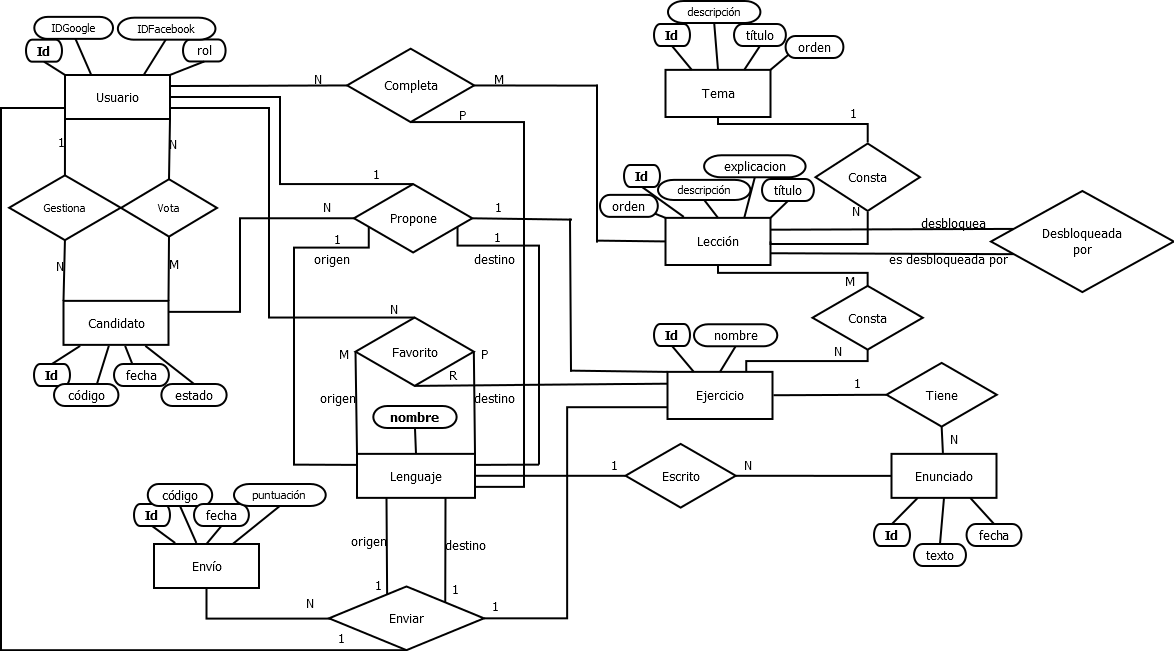
\includegraphics[width=\paperwidth]{images/bd-tfg}}
\caption{Modelo entidad-relacion\label{fig:ent_rel}}
\end{center}
\end{sidewaysfigure}

\begin{figure}
\begin{center}
\makebox[\textwidth]{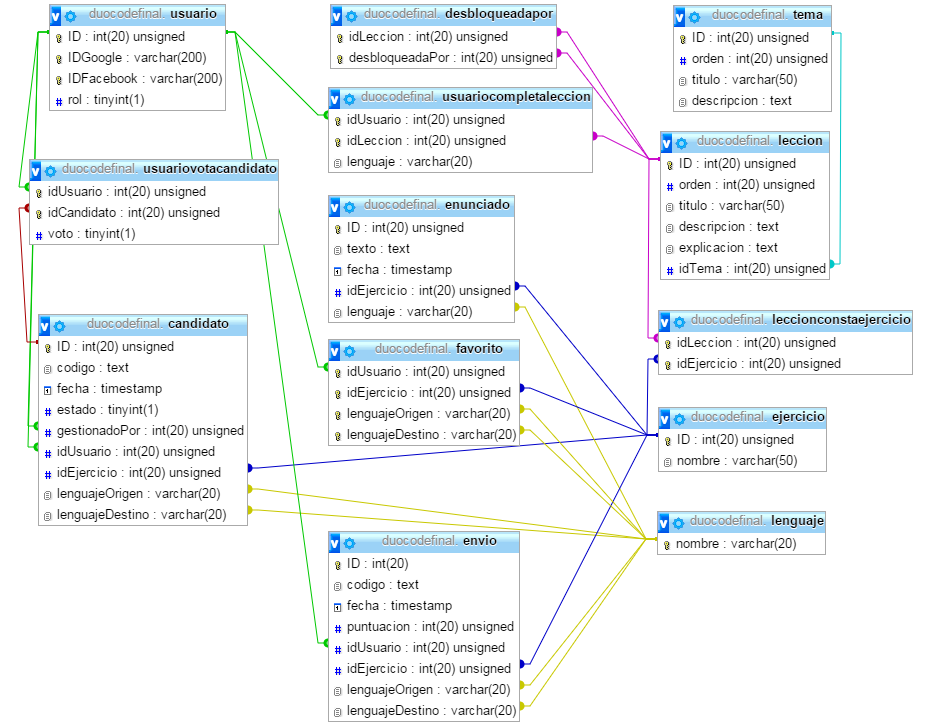
\includegraphics[scale=0.7]{images/bd}}
\caption{Modelo relacional\label{fig:rel}}
\end{center}
\end{figure}

\newpage

\textbf{Estructura de las tablas}

\begin{itemize}
\item Usuario: Tabla que contiene los datos de los usuarios. No hace falta guardar el nombre u otros datos personales ya que los obtenemos de la aplicación con la que haya iniciado sesión.


\begin{tabularx}{14cm}{|l|X|}
\hline
\textbf{Nombre} & \textbf{Descripción}                                                              \\ \hline
ID              & ID que le asigna la aplicación al usuario.                                         \\ \hline
IDGoogle        & ID que le asigna Google. Es opcional ya que el usuario puede iniciar con Facebook. \\ \hline
IDFacebook      & ID que le asigna Facebook. Es opcional ya que el usuario puede iniciar con Google. \\ \hline
\end{tabularx}
\vspace{1em}

\item UsuarioVotaCandidato: Tabla que contiene todos los votos de los usuarios a los candidatos.

\begin{tabularx}{14cm}{|l|X|}
\hline
\textbf{Nombre} & \textbf{Descripción}                                                              \\ \hline
IDUsuario       & ID del usuario que vota.                                                           \\ \hline
IDCandidato     & ID del candidato al que se quiere votar.                                           \\ \hline
Voto            & Puede tomar los valores 0 o 1 dependiendo de si el voto es positivo (1) o negativo (0). \\ \hline
\end{tabularx}
\vspace{1em}

\item Candidato: Tabla que contiene la información de los candidatos enviados por los usuarios de la aplicación.

\begin{tabularx}{14cm}{|l|X|}
\hline
\textbf{Nombre} & \textbf{Descripción}                                                              \\ \hline
ID              & Identificador único para el candidato.                                         \\ \hline
Código        & Texto propuesto como posible solución del ejercicio. \\ \hline
Fecha      & Fecha en la que se realiza la propuesta. \\ \hline
Estado              & Puede ser No Gestionado (0), Aceptado (1) o Rechazado (-1).                                         \\ \hline
GestionadoPor        & ID del usuario administrador que finalmente acepta o rechaza el candidato. Inicialmente se encuentra vacío. \\ \hline
IDUsuario      & ID del usuario que propone el candidato. \\ \hline
IDEjercicio              & ID del ejercicio que resuelve dicho candidato.                                         \\ \hline
LenguajeOrigen        & Lenguaje en el que se encuentra el enunciado del ejercicio. \\ \hline
LenguajeDestino      & Lenguaje en el que está la posible solución. \\ \hline
\end{tabularx}
\vspace{1em}

\item Tema: Tabla que contiene la información de los temas, primera división para organizar los ejercicios según a qué van dedicados. Los temas se conforman de una colección de lecciones.

\begin{tabularx}{14cm}{|l|X|}
\hline
\textbf{Nombre} & \textbf{Descripción}                                                              \\ \hline
ID       & ID propio del tema                                                           \\ \hline
Orden     & Orden en el que queremos que aparezca el tema.                                           \\ \hline
Título            & Nombre que distingue a los temas. \\ \hline
Descripción            & Texto breve que describe el tema. \\ \hline
\end{tabularx}
\vspace{1em}

\item Lección: Tabla que contiene la información de las lecciones, segunda división para la organización. Las lecciones se conforman de una serie de ejercicios y están incluidas en temas.

\begin{tabularx}{14cm}{|l|X|}
\hline
\textbf{Nombre} & \textbf{Descripción}                                                              \\ \hline
ID              & Identificador único para la lección.                                         \\ \hline
Orden        & Orden en el que queremos que aparezca la lección. \\ \hline
Título      & Nombre que distingue a las lecciones. \\ \hline
Descripción              & Texto breve que describe la lección.                                         \\ \hline
Expliciación        & Texto largo que sirve como introducción a la lección.  \\ \hline
IDTema      & ID del tema al que pertenece esta lección. \\ \hline
\end{tabularx}
\vspace{1em}

\item UsuarioCompletaLeccion: Tabla que contiene la relación de las lecciones con los usuarios que las han completado.

\begin{tabularx}{14cm}{|l|X|}
\hline
\textbf{Nombre} & \textbf{Descripción}                                                              \\ \hline
IDUsuario       & ID del usuario que ha completado la lección.                                                          \\ \hline
IDLección     & Lección que ha sido completada.                                           \\ \hline
Lenguaje            & Lenguaje en el que se ha completado dicha lección, ya que una lección puede ser completada por el mismo usuario en distintos lenguajes. \\ \hline
\end{tabularx}
\vspace{1em}

\item DesbloqueadaPor: Tabla que contiene la dependencia entre lecciones. Hay lecciones a las que solo se puede acceder si se han superado otras anteriormente.

\begin{tabularx}{14cm}{|l|X|}
\hline
\textbf{Nombre} & \textbf{Descripción}                                                              \\ \hline
IDLección       & ID de la lección a la que queremos asignar dependencia.                                                          \\ \hline
DesbloqueadaPor     & Lección que debe ser superada para poder acceder a la mencionada anteriormente.                                           \\ \hline
Lenguaje            & Lenguaje en el que se ha completado dicha lección, ya que una lección puede ser completada por el mismo usuario en distintos lenguajes. \\ \hline
\end{tabularx}
\vspace{1em}

\item Ejercicio: Tabla que contiene la información de los ejercicios existentes.

\begin{tabularx}{14cm}{|l|X|}
\hline
\textbf{Nombre} & \textbf{Descripción}                                                              \\ \hline
ID       & Identificador asignado por la aplicación para cada ejercicio. \\ \hline
Nombre     & Nombre con el que se diferenciará de los demás.                                           \\ \hline
\end{tabularx}
\vspace{1em}

\item LeccionConstaEjercicio: Tabla que contiene la relación donde se asignan los ejercicios a las correspondientes lecciones.

\begin{tabularx}{14cm}{|l|X|}
\hline
\textbf{Nombre} & \textbf{Descripción}                                                              \\ \hline
IDLección       & ID de la lección a la que se añade un ejercicio. \\ \hline
IDEjercicio     & ID del ejercicio añadido a la lección.                                           \\ \hline
\end{tabularx}
\vspace{1em}

\item Lenguaje: Tabla que contiene los lenguajes que podrán aprender los usuarios.

\begin{tabularx}{14cm}{|l|X|}
\hline
\textbf{Nombre} & \textbf{Descripción}                                                              \\ \hline
Nombre       & Nombre del lenguaje. \\ \hline
\end{tabularx}
\vspace{1em}

\item Enunciado: Tabla que contiene la información de los enunciados. Un enunciado es un código con un correspondiente lenguaje que forma parte de un ejercicio. Un ejercicio puede tener varios enunciados en varios idiomas.

\begin{tabularx}{14cm}{|l|X|}
\hline
\textbf{Nombre} & \textbf{Descripción}                                                              \\ \hline
ID       & ID que identifica al enunciado. \\ \hline
Texto     & Código, en lenguaje de origen, que tendrá que ser \emph{traducido}.                                           \\ \hline
Fecha     & Fecha en la que fue añadido el enunciado.                                           \\ \hline
IDEjercicio     & ID del ejercicio al que corresponde este enunciado.                                           \\ \hline
Lenguaje     & Lenguaje en el que está escrito el código de dicho enunciado.                                           \\ \hline
\end{tabularx}
\vspace{1em}

\item Favorito: Tabla que contiene la relación entre los usuarios y los ejercicios favoritos de estos.

\begin{tabularx}{14cm}{|l|X|}
\hline
\textbf{Nombre} & \textbf{Descripción}                                                              \\ \hline
IDUsuario       & ID del usuario que añade un ejercicio a favorito. \\ \hline
IDEjercicio     & ID del ejercicio que ha sido marcado como favorito. \emph{traducido}                                           \\ \hline
LenguajeOrigen     & Lenguaje del enunciado que ha sido marcado como favorito.                                           \\ \hline
LenguajeDestino     & Lenguaje que el usuario quería aprender al marcar este ejercicio como favorito.                                           \\ \hline
\end{tabularx}
\vspace{1em}

\item Envío: Tabla que contiene la relación entre los usuarios y todos los ejercicios que han realizado en la aplicación.

\begin{tabularx}{14cm}{|l|X|}
\hline
\textbf{Nombre} & \textbf{Descripción}                                                              \\ \hline
ID       & ID correspondiente a cada envío. \\ \hline
Código     & Código respuesta del usuario. \emph{traducido}                                           \\ \hline
Fecha     & Fecha en la que se ha resuelto el ejercicio.                                           \\ \hline
Puntuación     & Puntuación obtenida.                                           \\ \hline
IDUsuario     & Usuario que ha realizado el envío.                                           \\ \hline
IDEjercicio     & Ejercicio resuelto.                                           \\ \hline
LenguajeOrigen     & Lenguaje inicial del enunciado.                                           \\ \hline
LenguajeDestino     & Lenguaje en el que el usuario ha enviado el ejercicio.                                           \\ \hline
\end{tabularx}

\end{itemize}

\newpage
{\small
\bibliographystyle{abbrv}
\bibliography{tfg_bib}
}


\newpage
\appendix

\section{Especificación de requisitos} \label{app:Req}
%!TEX root = memoria_duocode_interfaz.tex

\subsection{localhost/duocode/rest/temas}
\textbf{REQ01 - GET:} No hace falta enviarle ninguna información. Devuelve la lista de todos los temas existentes en modo URL.

\begin{itemize}
\item[•] Response:
\{'temas": ['localhost/duocode/rest/temas/1 ', 'localhost/duocode/rest/temas/2 ']\}
\end{itemize}

\textbf{REQ02 – POST:} Con el post creamos un tema nuevo. Por una parte le pasamos por Payload la información del tema que queremos crear (título, descripción y orden en el que queremos que se muestre): 
\begin{itemize}
\item[•]Payload: 
\{'titulo': 'Bucles', 'descripcion': 'En este tema veremos bucles while y for…', 'orden': '2'\} \vspace{1em}

Por otra parte le enviamos por Header el ID del usuario, el token y el network, que nos sirven para comprobar que el usuario es administrador y tiene permisos para hacer esta operación:
\item[•]Header:
\{'idUsuario': '2', 'token': 'token', 'network': 'network'\}
\vspace{1em}

La respuesta que obtenemos está conformada por “error” e “id”, si la respuesta en el campo “error” es afirmativa significa que algo ha fallado y no ha podido terminar la operación correctamente, en este caso el id será “-1” ya que no ha sido asignado ninguno; si es negativa todo ha ido correctamente y el id será el asignado a este nuevo recurso. Un caso de error podría ser que el usuario no tenga los permisos necesarios.
\item[•]Response:
\{'error': 'no', 'id': '4'\}
\{'error': 'si', 'id': '-1'\}

\end{itemize}

\subsection{localhost/duocode/rest/temas/idTema}

En estos requisitos obtenemos el ID del tema mediante la URL.
\vspace{1em}

\textbf{REQ03 – POST:} Nos devuelve los datos y las lecciones que tiene el tema.

\begin{itemize}
\item[•]Response:
\{'titulo': 'Bucles', 'descripcion': 'En este tema veremos bucles while y for…', 'fechaCreacion': '17/11/2014', 'lecciones': ['localhost/duocode/rest/lecciones/1', 'localhost/duocode/rest/lecciones/2'], 'orden': '2'\}
\end{itemize}

\textbf{REQ04 – PUT:} Modificamos el tema en su totalidad.
\begin{itemize}
\item[•]Payload:
\{'titulo': 'tituloTema', 'descripcion': 'descripcionTema', 'orden': 'int con el orden en el que lo quieres mostrar'\}
\vspace{1em}

Enviamos por Header el ID del usuario, el token y el network, que nos sirven para comprobar que el usuario es administrador y tiene permisos para hacer esta operación:

\item[•]Header: 
\{'idUsuario': '2', 'token': 'token', 'network': 'network'\}
\vspace{1em}

La respuesta que obtenemos está conformada por “error”, en caso afirmativo significa que algo ha fallado y no ha podido terminar la operación correctamente; en caso negativo todo ha ido correctamente. Un caso de error podría ser que el usuario no tenga los permisos necesarios.
\item[•]Response: 
\{'error': 'no'\}
\end{itemize}

\textbf{REQ05 – DELETE:} Borramos el tema completamente. Enviamos por Header el ID del usuario, el token y el network, que nos sirven para comprobar que el usuario es administrador y tiene permisos para hacer esta operación:
\begin{itemize}
\item[•]Header:
\{'idUsuario': '2', 'token': 'token', 'network': 'network'\}
\vspace{1em}

La respuesta que obtenemos está conformada por “error”, en caso afirmativo significa que algo ha fallado y no ha podido terminar la operación correctamente; en caso negativo todo ha ido correctamente. Un caso de error podría ser que el usuario no tenga los permisos necesarios.
\item[•]Response: 
\{'error': 'no'\}
\end{itemize}

\subsection{localhost/duocode/rest/lecciones/}
\textbf{REQ06 – GET:} No hace falta enviarle ninguna información. Devuelve la lista de todas las lecciones existentes en modo URL. 
\begin{itemize}
\item[•]Response:
\{'lecciones': ['localhost/duocode/rest/lecciones/1', 'localhost/duocode/rest/lecciones/2']\}
\end{itemize}

\textbf{REQ07 – POST:} Con el post creamos una nueva lección. Por una parte le pasamos por Payload la información de la lección que queremos crear (título, descripción, explicación que aparecerá al inicio de ésta, orden en el que queremos que se muestre, ID del tema al que pertenecerá, un array de ejercicios que compondrán la lección y otro array de lecciones de las que depende para ser desbloqueada):

\begin{itemize}
\item[•]Payload: 
\{'titulo': 'tituloLeccion', 'descripcion': 'descripcionLeccion', 'explicacion': 'explicacion detallada', 'orden': '4', 'idTema': '1', 'idEjercicios': ['8', '14'], 'leccionesDesbloqueadoras': ['1', '2']\}
\vspace{1em}

Por otra parte le enviamos por Header el ID del usuario, el token y el network, que nos sirven para comprobar que el usuario es administrador y tiene permisos para hacer esta operación:
\item[•]Header: 
\{'idUsuario': '2', 'token': 'token', 'network': 'network'\}
\vspace{1em}

La respuesta que obtenemos está conformada por “error” e “id”, si la respuesta en el campo “error” es afirmativa significa que algo ha fallado y no ha podido terminar la operación correctamente, en este caso el id será “-1” ya que no ha sido asignado ninguno; si es negativa todo ha ido correctamente y el id será el asignado a esta nueva lección. Un caso de error podría ser que el usuario no tenga los permisos necesarios.
\item[•]Response: 
\{'error': 'no', 'id': '3'\}
\{'error': 'si', 'id': '-1'\}
\end{itemize}

\subsection{localhost/duocode/rest/lecciones/idLeccion}
En estos requisitos obtenemos el ID del candidato mediante la URL.
\vspace{1em}


\textbf{REQ08 – GET:} Nos devuelve los datos de la lección, y los ejercicios que tiene la lección.
\begin{itemize}

\item[•]Response:
\{ 'titulo': 'título de la lección (ej. Bucles fácil)', 'descripcion': 'descripción de la lección (ej. primeros bucles para practicar)', 'explicacion': 'explicación detallada', 'fechaCreacion': '17/11/2014', 'ejercicios': ['localhost/duocode/rest/ejercicios/2', 'localhost/duocode/ejercicios/3'], 'leccionesDesbloqueadoras': ['1', '2'], 'orden': '3'\}
\end{itemize}

\textbf{REQ09 – PUT:} Modificamos una lección. Aparte de cambiar los datos de una lección, en este método también podremos marcar como completada la lección para un usuario en un determinado lenguaje por lo que tenemos dos posibles Payloads:

\begin{itemize}
\item[•]Payload para modificar lección:
\{'leccion' : \{'titulo': 'tituloLeccion', 'descripcion': 'descripcionLeccion', 'explicacion':'explicacion detallada', 'idEjercicios': ['1', '2'], 'leccionesDesbloqueadoras': ['2', '3'], 'orden': '2', 'idTema': '1'\} \}

\item[•]
Payload para marcar como lección completada para un usuario:
\{'idUsuarioCompletaLeccion' : '3', 'lenguajeCompletadoLeccion' : 'Java', 'leccion' : \{'titulo': ' tituloLeccion ', 'descripcion': ' descripcionLeccion', 'explicacion':'explicacion detallada', 'idEjercicios': ['1', '2'], 'leccionesDesbloqueadoras': ['2', '3'], 'orden': '2', 'idTema': '1'\} \}

\vspace{1em}
Enviamos por Header el ID del usuario, el token y el network, que nos sirven para comprobar que el usuario es administrador y tiene permisos para hacer esta operación:

\item[•]Header:
\{'idUsuario': '2', 'token': 'token', 'network': 'network'\}
\vspace{1em}

La respuesta que obtenemos está conformada por “error”, en caso afirmativo significa que algo ha fallado y no ha podido terminar la operación correctamente; en caso negativo todo ha ido correctamente. Un caso de error podría ser que el usuario no tenga los permisos necesarios.
\item[•]Response: 
\{'error': 'no'\}
\end{itemize}

\textbf{REQ10 – DELETE:} Borramos la leccion completamente.Enviamos por Header el ID del usuario, el token y el network, que nos sirven para comprobar que el usuario es administrador y tiene permisos para hacer esta operación:
\begin{itemize}

\item[•]
Header: 
\{'idUsuario': '2', 'token': 'token', 'network': 'network'\}
\vspace{1em}

La respuesta que obtenemos está conformada por “error”, en caso afirmativo significa que algo ha fallado y no ha podido terminar la operación correctamente; en caso negativo todo ha ido correctamente. Un caso de error podría ser que el usuario no tenga los permisos necesarios.

\item[•] 
Response: 
\{'error': 'no'\}
\end{itemize}

\subsection{localhost/duocode/rest/ejercicios}
\textbf{REQ11 – GET:} No hace falta enviarle ninguna información. Devuelve la lista de todos los ejercicios existentes en modo URL.

\begin{itemize}
\item[•]
Response: 
\{'ejercicios': ['localhost/duocode/rest/temas/ejercicios/1', 'localhost/duocode/rest/ejercicios/2']\}
\end{itemize}

\textbf{REQ12 – POST:} Creamos un ejercicio nuevo. Por una parte le pasamos el nombre y los enunciados (un mismo ejercicio puede tener varios enunciados porque cada uno corresponde a distintos lenguajes de programación)

\begin{itemize}
\item[•]
Payload: 
\{'nombre': 'nombreDelEjercicio', 'enunciados': [“1”, “2”]\}
\vspace{1em}
Por otra parte le enviamos por Header el ID del usuario, el token y el network, que nos sirven para comprobar que el usuario es administrador y tiene permisos para hacer esta operación:

\item[•]
Header: 
\{'idUsuario': '2', 'token': 'token', 'network': 'network'\}

\vspace{1em}
La respuesta que obtenemos está conformada por “error” e “id”, si la respuesta en el campo “error” es afirmativa significa que algo ha fallado y no ha podido terminar la operación correctamente, en este caso el id será “-1” ya que no ha sido asignado ninguno; si es negativa todo ha ido correctamente y el id será el asignado a este nuevo recurso. Un caso de error podría ser que el usuario no tenga los permisos necesarios.

\item[•]
Response: 
\{'error': 'no', 'id': '4'\}
\{'error': 'si', 'id': '-1'\}
\end{itemize}

\subsection{localhost/duocode/rest/ejercicios/idEjercicio}
En estos requisitos obtenemos el ID del ejercicio mediante la URL.
El get nos devuelve los datos del ejercicio, y los enunciados que tiene el ejercicio (con el id de los lenguajes asociados)
\vspace{1em}

\textbf{REQ13 – GET:} Nos devuelve los datos del ejercicio, los enunciados que tiene y el nombre del lenguaje asociado a cada uno.

\begin{itemize}
\item[•]
Response: \{'nombre': 'nombreDelEjercicio', 'fechaCreacion': '17/11/2014', 'enunciados': [\{'enunciado':'localhost/duocode/rest/enunciados/5', 'nombreLenguaje': 'Java'\}, \{'enunciado':'localhost/duocode/rest/enunciados/8', 'nombreLenguaje': 'C++'\}]\}

\vspace{1em}
Con el delete borramos un ejercicio completamente
\end{itemize}

\textbf{REQ14 – DELETE:} Borramos un ejercicio completamente. Enviamos por Header el ID del usuario, el token y el network, que nos sirven para comprobar que el usuario es administrador y tiene permisos para hacer esta operación:

\begin{itemize}
\item[•]
Header: 
\{'idUsuario': '2', 'token': 'token', 'network': 'network'\}
\vspace{1em}

La respuesta que obtenemos está conformada por “error”, en caso afirmativo significa que algo ha fallado y no ha podido terminar la operación correctamente; en caso negativo todo ha ido correctamente. Un caso de error podría ser que el usuario no tenga los permisos necesarios.
\item[•]
Response: 
\{'error': 'no'\}
\end{itemize}

\subsection{localhost/duocode/rest/enunciados}
\textbf{REQ15 – GET:} No hace falta enviarle ninguna información. Devuelve la lista de todos los enunciados existentes en modo URL. 

\begin{itemize}
\item[•]
Response:
\{'enunciados': [\{'enunciado':'localhost/duocode/rest/enunciados/1', 'nombreLenguaje': 'Java'\}, \{'enunciado':'localhost/duocode/rest/enunciados/2', 'nombreLenguaje': 'C++'\}]\}
\vspace{1em}

\end{itemize}

\textbf{REQ16 – POST:} Creamos un enunciado nuevo. Por una parte le pasamos el lenguaje, el código y el ID del ejercicio correspondiente:

\begin{itemize}
\item[•]
Payload: 
\{'nombreLenguaje': 'Java', 'codigo': 'codigo del enunciado', 'idDelEjercicioQueResuelve': '1'\}
\vspace{1em}

Por otra parte le enviamos por Header el ID del usuario, el token y el network, que nos sirven para comprobar que el usuario es administrador y tiene permisos para hacer esta operación:

\item[•]
Header: 
\{'idUsuario': '2', 'token': 'token', 'network': 'network'\}
\vspace{1em}

La respuesta que obtenemos está conformada por “error” e “id”, si la respuesta en el campo “error” es afirmativa significa que algo ha fallado y no ha podido terminar la operación correctamente, en este caso el id será “-1” ya que no ha sido asignado ninguno; si es negativa todo ha ido correctamente y el id será el asignado a este nuevo enunciado. Un caso de error podría ser que el usuario no tenga los permisos necesarios.

\item[•]
Response: 
\{'error': 'no', 'id': '4'\} 
\{'error': 'si', 'id': '-1'\} 
\end{itemize}

\subsection{localhost/duocode/rest/enunciados/idEnunciado}
En estos requisitos obtenemos el ID del candidato mediante la URL.
\vspace{1em}


\textbf{REQ17 – GET:} Devuelve los datos del enunciado.

\begin{itemize}
\item[•]
Response: 
\{'fechaCreacion': '17/11/2014', 'codigo': 'codigo del enunciado a resolver', 'nombreLenguaje': 'Java', 'idDelEjercicioQueResuelve': '1'\}
\end{itemize}

\textbf{REQ18 – PUT:} Modificamos un enunciado.

\begin{itemize}
\item[•]
Payload: \{'nombreLenguaje': 'Java', 'codigo': 'código del enunciado', 'idDelEjercicioQueResuelve': '1'\}
\vspace{1em}

Enviamos por Header el ID del usuario, el token y el network, que nos sirven para comprobar que el usuario es administrador y tiene permisos para hacer esta operación:
\item[•]
Header: 
\{'idUsuario': '2', 'token': 'token', 'network': 'network'\}
\vspace{1em}

La respuesta que obtenemos está conformada por “error”, en caso afirmativo significa que algo ha fallado y no ha podido terminar la operación correctamente; en caso negativo todo ha ido correctamente. Un caso de error podría ser que el usuario no tenga los permisos necesarios.
\item[•]
Response: 
\{'error': 'no'\}
\end{itemize}

\textbf{REQ19 – DELETE:} Borramos un enunciado completamente. Enviamos por Header el ID del usuario, el token y el network, que nos sirven para comprobar que el usuario es administrador y tiene permisos para hacer esta operación:
\begin{itemize}
\item[•]
Header: 
\{'idUsuario': '2', 'token': 'token', 'network': 'network'\}
\vspace{1em}

La respuesta que obtenemos está conformada por “error”, en caso afirmativo significa que algo ha fallado y no ha podido terminar la operación correctamente; en caso negativo todo ha ido correctamente. Un caso de error podría ser que el usuario no tenga los permisos necesarios.
\item[•]
Response: 
\{'error': 'no'\}
\end{itemize}

\subsection{localhost/duocode/rest/lenguajes/}
\textbf{REQ20 – GET:} No hace falta enviarle ninguna información. Devuelve la lista de todos los lenguajes existentes. 
\begin{itemize}
\item[•]
Response: 
\{'lenguajes': [\{'nombre': 'Java'\}, \{'nombre': 'C++'\}]\}
\end{itemize}

\textbf{REQ21 – POST:} Creamos un lenguaje nuevo. La única información necesaria es el nombre.

\begin{itemize}
\item[•]
Payload: 
\{'nombre': 'Python'\}
\vspace{1em}

Por otra parte le enviamos por Header el ID del usuario, el token y el network, que nos sirven para comprobar que el usuario es administrador y tiene permisos para hacer esta operación:

\item[•]
Header: 
\{'idUsuario': '2', 'token': 'token', 'network': 'network'\}
\vspace{1em}

La respuesta que obtenemos está conformada por “error” y “nombreConfirmacion”, si la respuesta en el campo “error” es afirmativa significa que algo ha fallado y no ha podido terminar la operación correctamente; si es negativa todo ha ido correctamente y el “nombreConfirmacion” será el asignado a este nuevo lenguaje. Un caso de error podría ser que el usuario no tenga los permisos necesarios.

\item[•]
Response: 
\{'error': 'no', ' nombreConfirmacion ': 'Python'\}

\end{itemize}

\subsection{localhost/duocode/rest/candidatos/}
\textbf{REQ22 – GET:} No hace falta enviarle ninguna información. Devuelve la lista de todos los candidatos existentes en modo URL. 

\begin{itemize}
\item[•]
Response: 
\{'candidatos': ['localhost/duocode/rest/candidatos/1', 'localhost/duocode/rest/candidatos/2']\}
\end{itemize}

\textbf{REQ23 – POST:} Generamos un nuevo candidato, y le asociamos el usuario que lo ha creado. Por un lado le enviamos el código del candidato, el ID del ejercicio que resuelve, el lenguaje en el que está escrito el candidato y el lenguaje del enunciado:
\begin{itemize}
\item[•]
Payload: 
\{'codigo': 'codigoDelCandidato', 'idEjercicio': '4', 'nombreLenguajeDestino': 'Java', 'nombreLenguajeOrigen': 'C++'\}
\vspace{1em}

Por otra parte le enviamos por Header el ID del usuario, el token y el network, que nos sirven para saber qué usuario es el que ha enviado el candidato:
\item[•]
Header: 
\{'idUsuario': '2', 'token': 'token', 'network': 'network'\}
\vspace{1em}

La respuesta que obtenemos está conformada por “error” e “idCandidato”, si la respuesta en el campo “error” es afirmativa significa que algo ha fallado y no ha podido terminar la operación correctamente, en este caso el id será “-1” ya que no ha sido asignado ninguno; si es negativa todo ha ido correctamente y el id será el asignado a este nuevo enunciado. 
\item[•]
Response: 
\{'error': 'no', 'id': '4'\}
\end{itemize}

\subsection{localhost/duocode/rest/candidatos/idCandidato}
En estos requisitos obtenemos el ID del candidato mediante la URL.
\vspace{1em}

\textbf{REQ24 – GET:} Devuelve los datos de un candidato, incluidos los votos que tiene.

\begin{itemize}
\item[•]
Response: 
\{'idEjercicio': 'localhost/duocode/rest/ejercicios/4', 'nombreLenguajeOrigen' : 'Java', 'nombreLenguajeDestino : 'C++', 'codigo' : 'codigo del candidato', 'idUsuarioCreador' : '2', 'fechaCreacion': '17/11/2014', 'votos': [ \{idUsuarioVoto':'8', 'voto': 'pos'\}, \{idUsuarioVoto':'5', 'voto': 'neg'\} ] \}
\end{itemize}

\textbf{REQ25 – PUT:} Excepcionalmente no modificará todo el candidato, sino que servirá para que un usuario pueda votar, modificar el voto o eliminarlo (si se vuelve a votar positivo o negativo el voto se anula). Se envía el ID del usuario y el voto (1 si es positivo y 0 si es negativo).

\begin{itemize}
\item[•]
Payload: 
\{'votar': \{'idUsuario': 6, 'voto': 1\}\}
\vspace{1em}

La respuesta que obtenemos está conformada por 'error', en caso afirmativo significa que algo ha fallado y no ha podido terminar la operación correctamente; en caso negativo todo ha ido correctamente. 
\item[•]
Response: 
\{'error': 'no'\}
\end{itemize}

\textbf{REQ26 – DELETE:} Borramos un candidato completamente.

\begin{itemize}
\item[•]
Header: 
\{'idUsuario': '2', 'token': 'token', 'network': 'network'\}
\vspace{1em}

La respuesta que obtenemos está conformada por “error”, en caso afirmativo significa que algo ha fallado y no ha podido terminar la operación correctamente; en caso negativo todo ha ido correctamente. Un caso de error podría ser que el usuario no tenga los permisos necesarios.

\item[•]
Response: 
\{'error': 'no'\}
\end{itemize}

\subsection{localhost/duocode/rest/usuarios/}
El GET devuelve todos los usuarios, solo si lo pide un administrador (esta petición va con el ID de un usuario administrador y el token)
\textbf{REQ27 – GET:} Devuelve todos los usuarios. A diferencia de otros, este GET sólo lo puede hacer un administrador por lo que necesitamos nuevamente del Header.

\begin{itemize}
\item[•]
Header:
\{'idUsuario': '2', 'token': 'token', 'network': 'network'\}
\vspace{1em}

La respuesta que obtenemos está conformada por “error” y la lista de usuarios. Si “error” tiene una respuesta afirmativa, significa que algo ha fallado y no ha podido terminar la operación correctamente; en caso negativo todo ha ido correctamente y muestra la lista de usuarios mediante su URL. Un caso de error podría ser que el usuario no tenga los permisos necesarios.

\item[•]
Response: 
\{'error': 'no”, 'usuarios' : ['localhost/duocode/rest/usuario/1', 'localhost/duocode/rest/usuario/2'] \}
\end{itemize}

\subsection{localhost/duocode/rest/usuarios/idUsuario}
En estos requisitos obtenemos el ID del candidato mediante la URL.
\vspace{1em}

\textbf{REQ28 – GET:} Devuelve la información asociada a un usuario. Enviamos por Header el ID del usuario, el token y el network, que nos sirven para comprobar que el usuario que accede es el mismo del que se da la información:

\begin{itemize}
\item[•]
Header: 
\{'idUsuario': '2', 'token': 'token', 'network': 'network'\}
\vspace{1em}

La respuesta es la información detallada de toda la sesión del usuario
\item[•]
Response: \{'nick' : 'nickDelUsuairo',
'leccionesCompletadas' : ['localhost/duocode/rest/lecciones/1', 'localhost/duocode/rest/lecciones/2'],
'favoritos': [\{'ejercicio' : 'localhost/duocode/rest/ejercicios/5', 'nombreLenguajeOrigien': 'Java', 'nombreLenguajeDestino': 'C++'\}, \{'ejercicio' : 'localhost/duocode/rest/ejercicios/7', 'nombreLenguajeOrigien': 'Python', 'nombreLenguajeDestino': 'C++'\}],
'historialEjercicios' : [\{'idEnvio': '1', 'ejercicio' : 'localhost/duocode/rest/ejercicios/4', 'nombreLenguajeOrigien': 'Java', 'nombreLenguajeDestino': 'C++', 'codigo': 'codigo enviado', 'fecha': '17/11/2014', 'puntuacion' : '2'\}, \{'idEnvio': '2', 'ejercicio' : 'localhost/duocode/rest/ejercicios/9', 'nombreLenguajeOrigien': 'Python', 'nombreLenguajeDestino': 'Perl', 'codigo': 'codigo enviado', 'fecha': '18/11/2014', 'puntuacion' : '7'\}],
'candidatosPropuestos': ['localhost/duocode/rest/candidatos/18', 'localhost/duocode/rest/candidatos/23'] \}
\end{itemize}

\textbf{REQ29 – DELETE}: Borramos un usuario completamente.
Enviamos por Header el ID del usuario, el token y el network, que nos sirven para comprobar que el usuario es administrador y tiene permisos para hacer esta operación:

\begin{itemize}
\item[•]
Header: 
\{'idUsuario': '2', 'token': 'token', 'network': 'network'\}
\vspace{1em}

La respuesta que obtenemos está conformada por “error”, en caso afirmativo significa que algo ha fallado y no ha podido terminar la operación correctamente; en caso negativo todo ha ido correctamente. Un caso de error podría ser que el usuario no tenga los permisos necesarios.

\item[•]
Response: 
\{'error': 'no'\}
\end{itemize}

\subsection{localhost/duocode/rest/envios}
\textbf{REQ30 – GET}: Devuelve todos los envíos para que un administrador pueda tener información de ellos. Como sólo puede tener acceso a esto el administrador, es necesaria la siguiente información:

\begin{itemize}
\item[•]
Header: 
\{'idUsuario': '2', 'token': 'token', 'network': 'network'\}
\vspace{1em}

La respuesta se compone de usuarios con historiales de ejercicios.

\item[•]
Response: \{ 'envios' : [ \{'idUsuario': '1', 'historialEjercicios' : [\{'idEnvio': '1', 'ejercicio' : 'localhost/duocode/rest/ejercicios/5', 'nombreLenguajeOrigien': 'Java', 'nombreLenguajeDestino': 'C++', 'codigo': 'codigo enviado', 'fecha': '17/11/2014', 'puntuacion' : '2'\}, \{'idEnvio': '2', 'ejercicio' : 'localhost/duocode/rest/ejercicios/7', 'nombreLenguajeOrigien': 'Python', 'nombreLenguajeDestino': 'Perl', 'codigo': 'codigo enviado', 'fecha': '18/11/2014', 'puntuacion' : '7'\}]\},
\{'idUsuario': '4', 'historialEjercicios' : [\{'idEnvio': '1', 'ejercicio' : 'localhost/duocode/rest/ejercicios/6', 'nombreLenguajeOrigien': 'Java', 'nombreLenguajeDestino': 'C++', 'codigo': 'codigo enviado', 'fecha': '17/11/2014', 'puntuacion' : '2'\}, \{'idEnvio': '2', 'ejercicio' : 'localhost/duocode/rest/ejercicios/5', 'nombreLenguajeOrigien': 'Python', 'nombreLenguajeDestino': 'Perl', 'codigo': 'código enviado', 'fecha': '18/11/2014', 'puntuacion' : '7'\}]\} ] \}
\end{itemize}

\textbf{REQ31 – PUT:} Corregimos un ejercicio, y también se comprobará si se ha completado la lección y en caso afirmativo se marcará como completada en la BD. Por una parte enviamos la URL del ejercicio, el lenguaje del enunciado, el lenguaje de la solución y el código.

\begin{itemize}
\item[•]
Payload: 
\{'ejercicio': 'localhost/duocode/rest/ejercicios/idEjercicio1', 'nombreLenguajeOrigien': 'Java', 'nombreLenguajeDestino': 'C++', 'codigo': 'codigo enviado en el lenguaje de destino'\} 
\vspace{1em}

Por otra parte enviamos el idUsuaro, token y network para comprobar que el usuario que envía el ejercicio para corregir es el que tiene la sesión iniciada.
\item[•]
Header: \{'idUsuario': 'idDelUsuario', 'token': 'token', 'network': 'network'\}
\vspace{1em}

La respuesta que obtenemos está conformada por “error” y “puntuacion”. Si “error” tiene un valor afirmativo significa que algo ha fallado y no ha podido terminar la operación correctamente; en caso negativo todo ha ido correctamente y devuelve la puntuación que ha obtenido el ejercicio al ser corregido. Un caso de error podría ser que el usuario no coincida.
\item[•]
Response: \{'error': 'no', 'puntuacion': '2'\}
\end{itemize}


\newpage
\section{Manual de instalación}
En este apartado se detallan los pasos a seguir para tener instalado \textbf{DuoCode} en un sistema \textit{Linux}, con el fin de poder trabajar directamente con los ficheros fuentes y extender el proyecto. La dirección donde podemos descargar todo el código es \url{https://github.com/jucallej/DuoCode.git}.

El software necesario para trabajar con el proyecto se especifica a continuación.

\begin{itemize}
\item \textbf{Requisitos generales}
\begin{itemize}
\item Java 7.
\item Git.
\item Navegador Web - Google Chrome.
\end{itemize}
\end{itemize}
\begin{itemize}
\item \textbf{Requisitos para el Servicio Web}
\begin{itemize}
\item Xampp.
\item Tomcat 8.0.
\item NetBeans 8.0.
\end{itemize}
\end{itemize}
\begin{itemize}
\item \textbf{Requisitos para el Front-End}

\begin{itemize}
\item Soporte SSL en Xampp y Tomcat.
\end{itemize}
\end{itemize}
\begin{itemize}
\item \textbf{Requisitos para la Aplicación móvil}
\begin{itemize}
\item Node.Js 0.10.X.
\item Phonegap 5.0.0.
\item Eclipse Luna con plugin para Android.
\end{itemize}
\end{itemize}

\subsection{Instalación de desarrollador}

Es importante seguir el orden de instalación que aparece a continuación para no tener problemas de dependencias entre programas. 

\begin{itemize}
\item \textbf{Java}

En primer lugar necesitamos tener instalada una versión de Java. La forma más sencilla es acceder a la web \url{http://www.java.com/es/} y descargar la última versión.

Es posible usar el siguiente comando en el termina:
{\codesize
\begin{verbatim}
$ sudo apt-get install openjdk-7-jdk openjdk-7-jre
\end{verbatim}
}


\item \textbf{Git}

Para poder descargar todos los ficheros fuentes del proyecto es necesario tener un cliente Git instalado y configurado.

Una opción es acceder a la web \url{http://git-scm.com/downloads/guis} y elegir el cliente que queramos. 

Es posible usar el siguiente comando en el termina:

{\codesize
\begin{verbatim}
$ sudo apt-get install git
\end{verbatim}
}

Una vez instalado git podemos clonar el proyecto \textbf{DuoCode} y obtener una copia en nuestro sistema. Si trabajas con un cliente gráfico simplemente hay que pinchar en el botón \textit{clone} y escribir la dirección del repositorio \url{https://github.com/jucallej/DuoCode.git}.

También podemos clonar el proyecto directamente desde la línea de comandos:
{\codesize
\begin{verbatim}
$ git clone https://github.com/jucallej/DuoCode.git
\end{verbatim}
}


\item \textbf{Google Chrome}

Cualquier navegador es válido pero Chrome cuenta con un plugin (Advance Rest Client) que es necesario para hacer pruebas con el servicio REST. Para instalar el navegador accedemos a la web de Chrome \url{https://www.google.es/chrome/} y pinchamos en el botón de descarga.

Es posible usar el siguiente comando en el termina:
{\codesize
\begin{verbatim}
$ sudo apt-get install google-chrome-stable
\end{verbatim}
}



\item \textbf{XAMPP}

Es necesario tener instalado un servidor local. XAMPP nos proporciona una base de datos MySQL y un servidor Apache.
Para instalarlo solo hay que acceder a la web \url{https://www.apachefriends.org/index.html} y descargar la última versión disponible.


Una vez instalado y funcionando accedemos a \url{http://localhost/phpmyadmin} para importar la Base de datos.
Creamos una Base de datos nueva con el nombre `Duocode', la seleccionamos e importamos el archivo 'Duocode.sql' para que nos cree las tablas y cargue la información del proyecto.


En la carpeta \textit{`htdocs'}, que se encuentra dentro de la carpeta del servidor XAMPP, es donde tenemos que poner la parte del front-end.
Copiamos la carpeta \textit{`duocode'} que contiene el \textit{`index.html'} y todos los scripts y la pegamos en \textit{`htdocs'}.
Podemos probar el funcionamiento accediendo a la dirección \url{`http://localhost/duocode'}.



\item \textbf{Tomcat}

Para el servicio web REST necesitamos tener instalado Tomcat 8.0 o superior. Para ello, accedemos a la web \url{http://tomcat.apache.org/download-80.cgi} (para la versión 8.0), descargamos la última versión para nuestro sistema operativo y lo descomprimimos.



\item \textbf{NetBeans}

El IDE que se ha usado para desarrollar el proyecto es NetBeans 8.0. Nos permite integrar el sistema de control de versiones \textit{Git} y los servidores. Se puede descargar desde la web \url{https://netbeans.org/downloads/}.

Una vez instalado importamos el proyecto descargado desde el Git y seleccionamos el servidor con el que queremos que funcione, en nuestro caso será el Tomcat descargado anteriormente.

Las bibliotecas necesarias se importan de manera automática una vez que hemos cargado el proyecto en NetBeans.

\item \textbf{Certificados SSL}

Para que tanto el front-end como el servicio web funcionen con \textit{https} es necesario activar SSL en los servidores \textit{Tomcat} y \textit{Apache} del XAMPP.

Hemos creado nuestros propios certificados SSL y se pueden encontrar en la carpeta \textit{duocode/certificados}. Ña contraseña es \textit{complutense}.

Tomcat lo podemos configurar gracias al archivo \textit{server.xml} encontrado en /apache-tomcat-8.0.21/conf/server.xml.
Lo abrimos y dentro del elemento:
{\codesize
\begin{verbatim}
 < Service name = 'Catalina' >  
\end{verbatim}
}
pegamos estas líneas de código (cambiando la ruta del proyecto):

{\codesize
\begin{verbatim}
<Connector port="8443" protocol="org.apache.coyote.http11.Http11NioProtocol"
               maxThreads="150" SSLEnabled="true" scheme="https" secure="true"
               clientAuth="false" sslProtocol="TLS"
           keystoreType="PKCS12"
           keystoreFile="{Ruta al repositorio}\DuoCode\duocode\certificados\mycert.p12" keystorePass="contraseña"/>
\end{verbatim}
}

Para configurar el server Apache que nos proporciona XAMPP primero tenemos que poner los archivos \textit{`mars-server.crt', `mars-server.key'} en la siguiente ruta:

\begin{itemize}


\item \textit{'/opt/lampp/etc/ssl.crt/'} los ficheros con la extensión .crt.

\item \textit{'/opt/lampp/etc/ssl.key/'} el fichero con la extensión .key.

\end{itemize}

Una vez tenemos los certificados y la clave en las rutas adecuadas editamos el fichero \textit{httpd-ssl.conf}. Dependiendo de la versión puede tener un aspecto u otro, en nuestro caso hemos definido un nuevo VirtualHost con la siguiente configuración.

{\codesize
\begin{verbatim}
<VirtualHost _default_:443>

DocumentRoot "/opt/lampp/htdocs"
ServerName localhost:443
ServerAdmin you@example.com
ErrorLog "/opt/lampp/logs/error_log"
TransferLog "/opt/lampp/logs/access_log"

SSLEngine on

SSLCertificateFile "/opt/lampp/etc/ssl.crt/mars-server.crt"
SSLCertificateKeyFile "/opt/lampp/etc/ssl.key/mars-server.key"
SSLCertificateChainFile "/opt/lampp/etc/ssl.crt/my-ca.crt"

SSLCACertificateFile "/opt/lampp/etc/ssl.crt/my-ca.crt"

<FilesMatch "\.(cgi|shtml|phtml|php)$">
    SSLOptions +StdEnvVars
</FilesMatch>
<Directory "/opt/lampp/cgi-bin">
    SSLOptions +StdEnvVars
</Directory>

BrowserMatch "MSIE [2-5]" \
         nokeepalive ssl-unclean-shutdown \
         downgrade-1.0 force-response-1.0

CustomLog "/opt/lampp/logs/ssl_request_log" \
          "%t %h %{SSL_PROTOCOL}x %{SSL_CIPHER}x \"%r\" %b"

<Directory "/opt/lampp/htdocs">
        Options Indexes
        AllowOverride None
        Allow from from all
        Order allow,deny
</Directory>

</VirtualHost>
\end{verbatim}
}

Una vez configurado podemos acceder a la dirección \url{https://localhost/duocode}, aunque nos saldrá un mensaje indicando que el certificado no está verificado (es un certificado que hemos creado nosotros) así que lo añadimos como excepción y ya tenemos \textbf{DuoCode} instalado.


\item \textbf{Node.js}

Para poder trabajar con PhoneGap - Cordova es necesario tener instalado Node.js en nuestro equipo. Podemos hacerlo descargándolo desde la web \url{`https://nodejs.org/'} o directamente desde un terminal:

{\codesize
\begin{verbatim}
$ sudo add-apt-repository ppa:chris-lea/node.js
$ sudo apt-get update
$ sudo apt-get install nodejs
\end{verbatim}
}

Es necesario que la versión sea 0.8+. Podemos comprobarlo tecleando desde el terminal: 

{\codesize
\begin{verbatim}
$ node -v
\end{verbatim}
}

\item \textbf{PhoneGap}

PhoneGap nos sirve para crear una app móvil desde el HTML5, CSS y JS de nuestro proyecto. Para instalarlo podemos descargarlo desde la web \url{http://phonegap.com} o directamente desde un terminal:

{\codesize
\begin{verbatim}
$ npm install -g phonegap
\end{verbatim}
}

\item \textbf{Eclipse y Android SDK}

Gracias al plugin de Android podemos usar Eclipse como IDE para probar la app móvil de DuoCode. Instalamos la última versión de Eclipse descargándolo desde la web \url{http://eclipse.org}.

Una vez descargado lo abrimos y vamos a añadir el plugin para Android.
Pinchamos en \textbf{help - Install New Software} y añadimos la siguiente URL \url{https://dl-ssl.google.com/android/eclipse/} y seleccionamos \textbf{next} hasta completar la instalación.

Reiniciamos Eclipse y tenemos que especificar la dirección del \textbf{Android SDK} que acabamos de descargar para que se actualice y tener Eclipse listo.

Podemos importar la carpeta del proyecto que encontramos en DuoCode y probarlo con el emulador seleccionando la carpeta del proyecto y pulsando sobre \textit{`Run'}.

\end{itemize}

\subsection{Desplegado modo desarrollador}

Finalmente, una vez instalado y configurado todo, podemos desplegar y trabajar sobre el proyecto local.

Tenemos que seguir una serie de pasos que se detallan a continuación:

\begin{itemize}

\item \textbf{Arranque de XAMPP}

Para arrancar el servidor Apache y tener acceso a la Base de datos es necesario que \textit{XAMPP} esté funcionando. Para ello abrimos un terminal, nos posicionamos en la carpeta donde se haya instalado \textit{`/opt/lampp/'} y escribimos el siguiente comando:
{\codesize
\begin{verbatim}
$ ./xampp start
\end{verbatim}
}
Es posible que se quede parado mientras intenta arrancar el servidor Apache porque necesite la contraseña del certificado. Si esto ocurre escribimos en el terminal \textit{`complutense'} y pulsamos Enter.



\item \textbf{Despliegue del servicio REST}

Para desplegar el servicio REST abrimos Netbeans y seleccionamos el proyecto DuoCode que importamos durante la instalación. Accedemos a \textit{Run} - \textit{Build} y después pulsamos con el botón derecho del ratón sobre la carpeta del proyecto y seleccionamos \textit{Deploy}.

Con estos pasos conseguimos que el servidor Tomcat se inicie y se despliegue el servicio REST.

\item \textbf{Acceso a DuoCode}

Si no se ha producido ningún problema durante la instalación y el despliegue podemos acceder a la web \url{https://localhost/duocode} y probar la aplicación.

\end{itemize}


\newpage
\appendix


%\input{divide_y_venceras}

\end{document}
